\section{Resultados}\label{sec:resultados}

\subsection{Features}\label{subsec:features}

Realizamos un \textit{scatter plot} de los datos, exponemos los resultados en la figura \ref{fig:trending}.

\begin{figure}[hbtp]
  \centering
  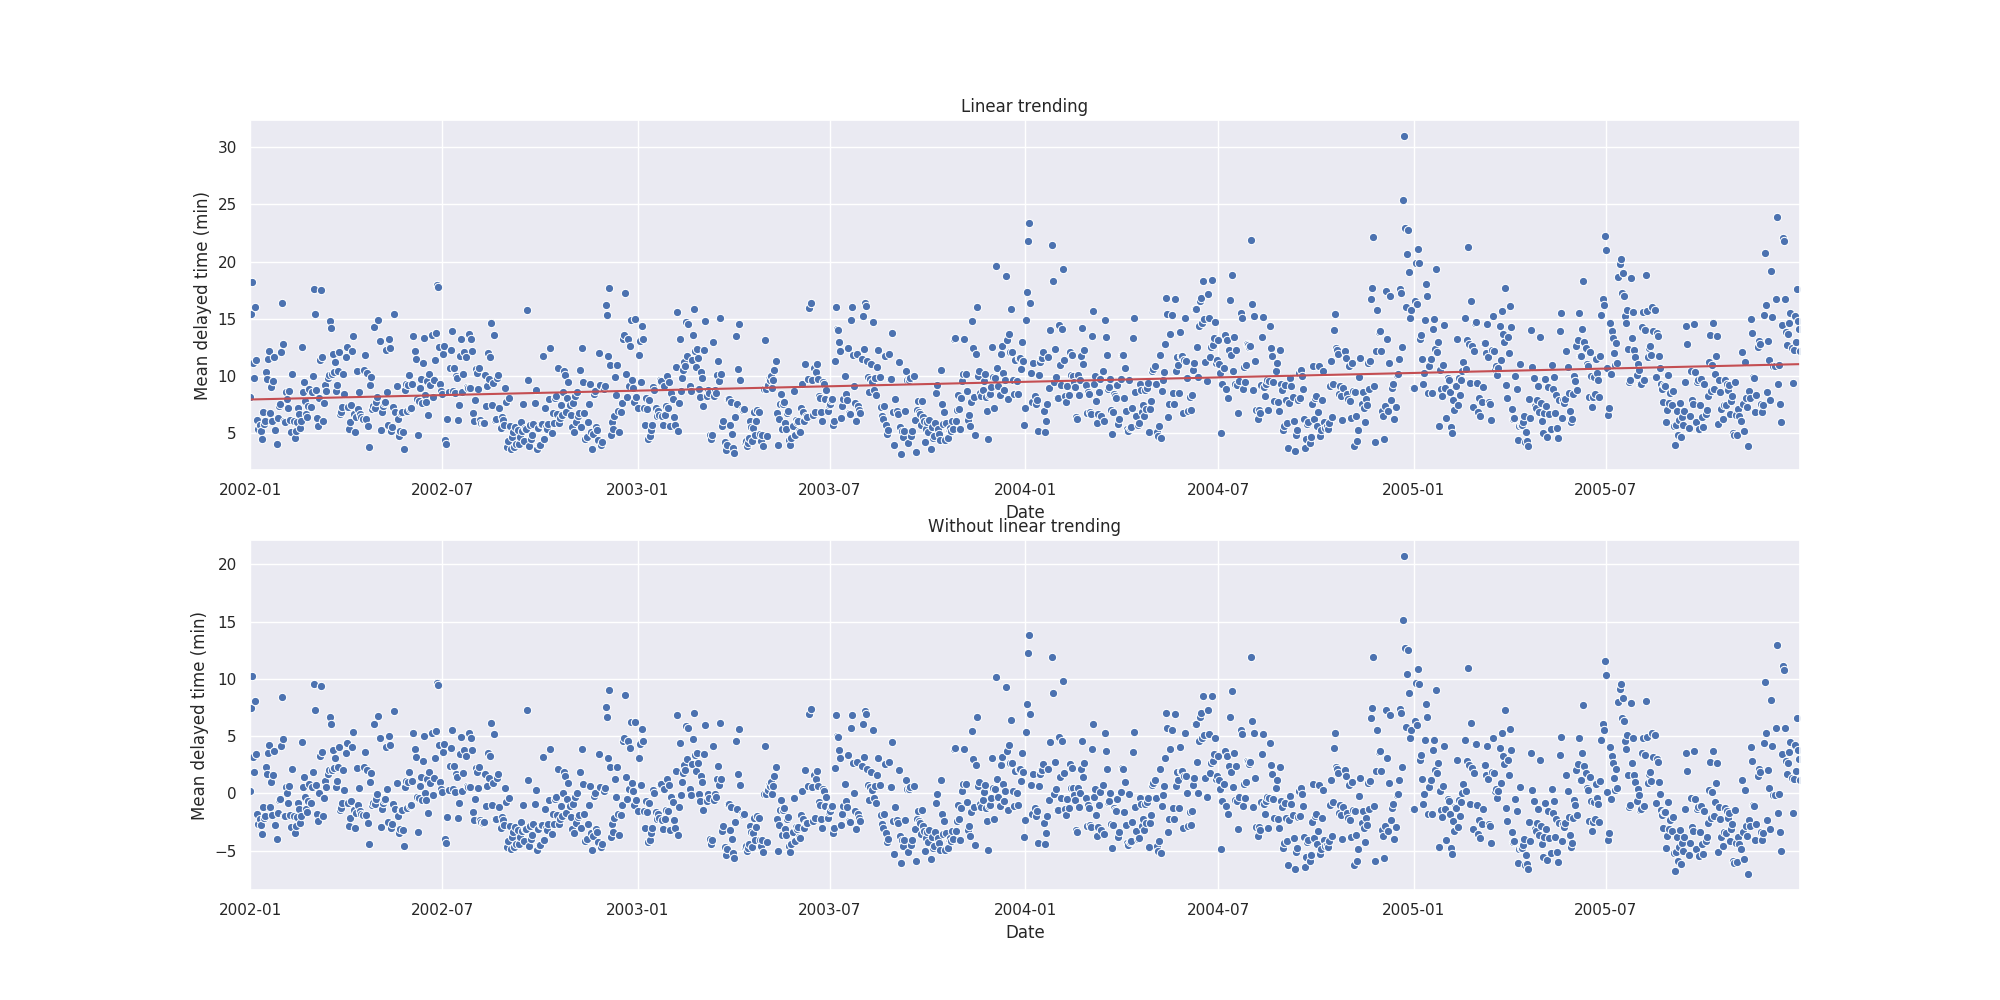
\includegraphics[width=\textwidth]{plots/linear_trending.png}
  \caption{\textit{Detrending} de los datos}
  \label{fig:trending}
\end{figure}

Realizamos un ajuste lineal de los datos, los que nos da un nuevo dataset con media cero (proceso conocido
como \textit{detrending}).

Luego, realizamos gr\'aficos que nos muestren c\'omo se comportan los retrasos dentro de los meses de un a\~no, los
d\'ias de un mes y los d\'ias de una semana. Exponemos los datos en las figuras \ref{fig:within_year}, \ref{fig:within_month}
y \ref{fig:within_week}.

\begin{figure}[hbtp]
  \centering
  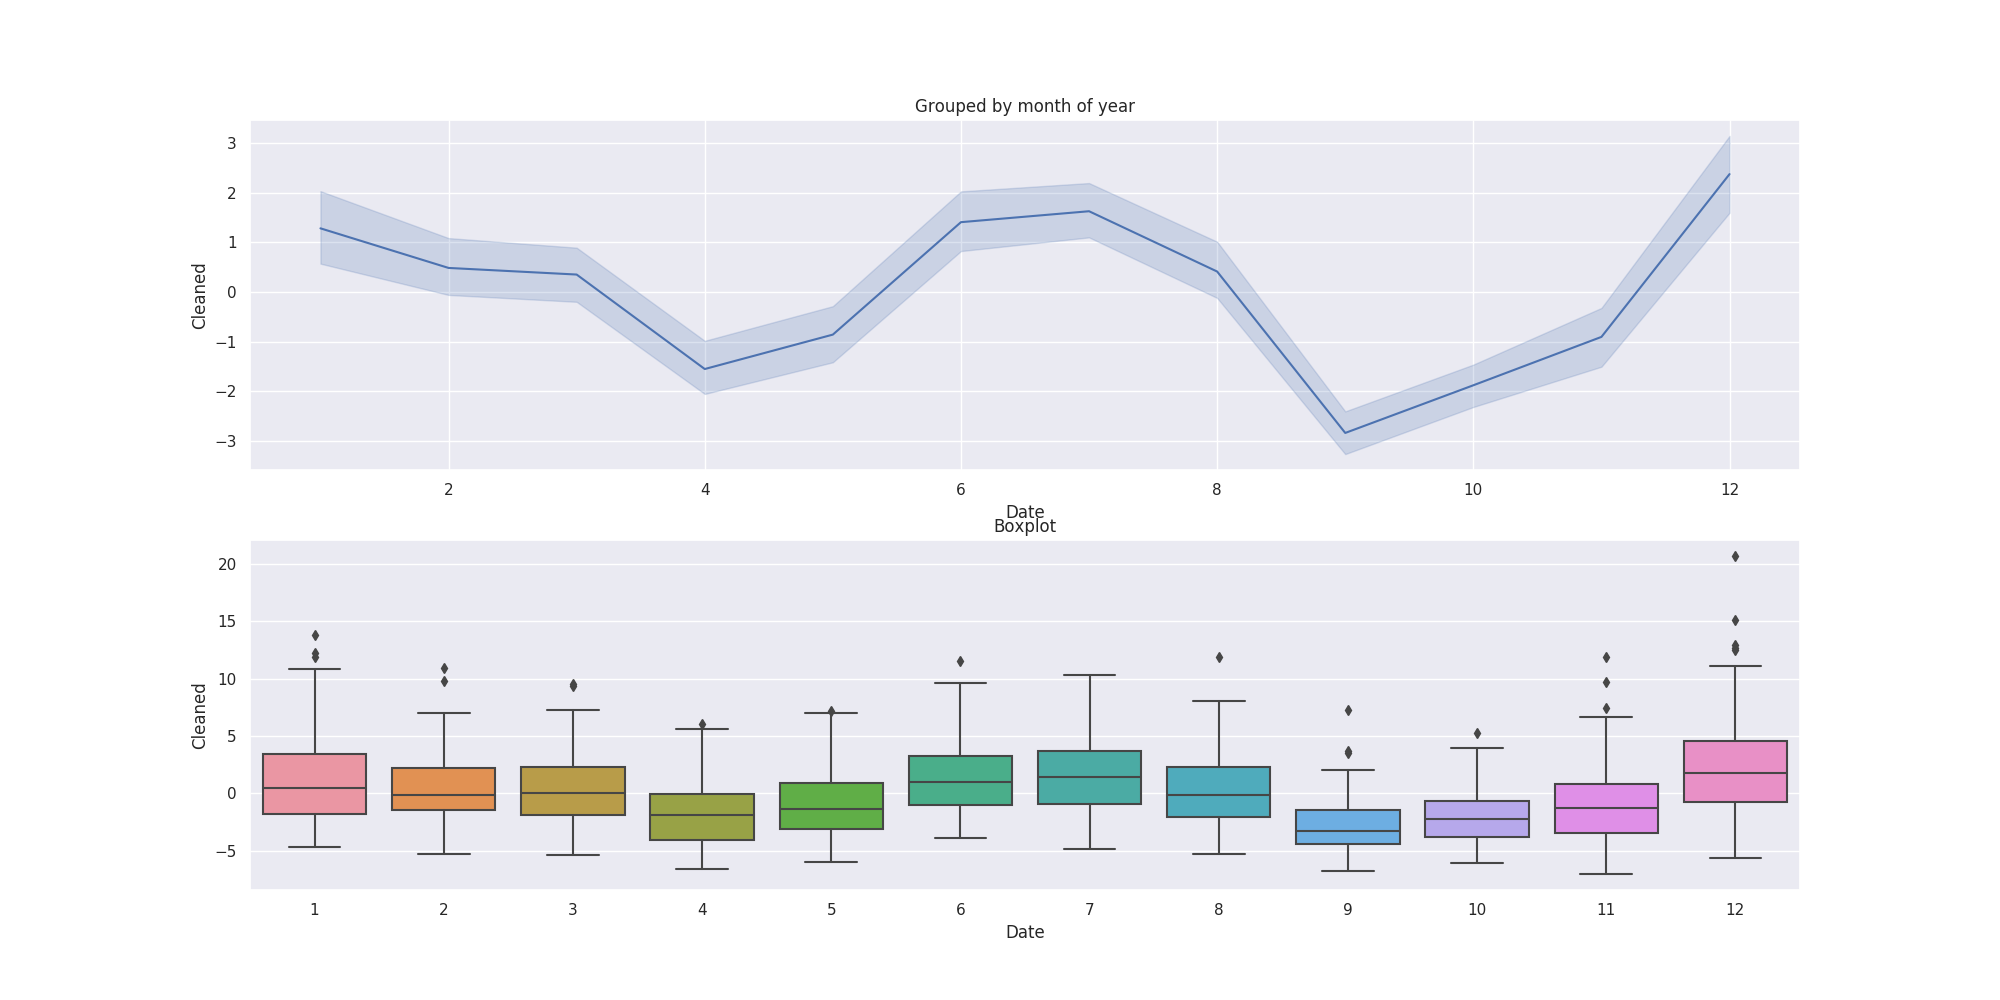
\includegraphics[width=0.7\textwidth]{plots/within_year.png}
  \caption{Retraso medio por mes}
  \label{fig:within_year}
\end{figure}

\begin{figure}[hbtp]
  \centering
  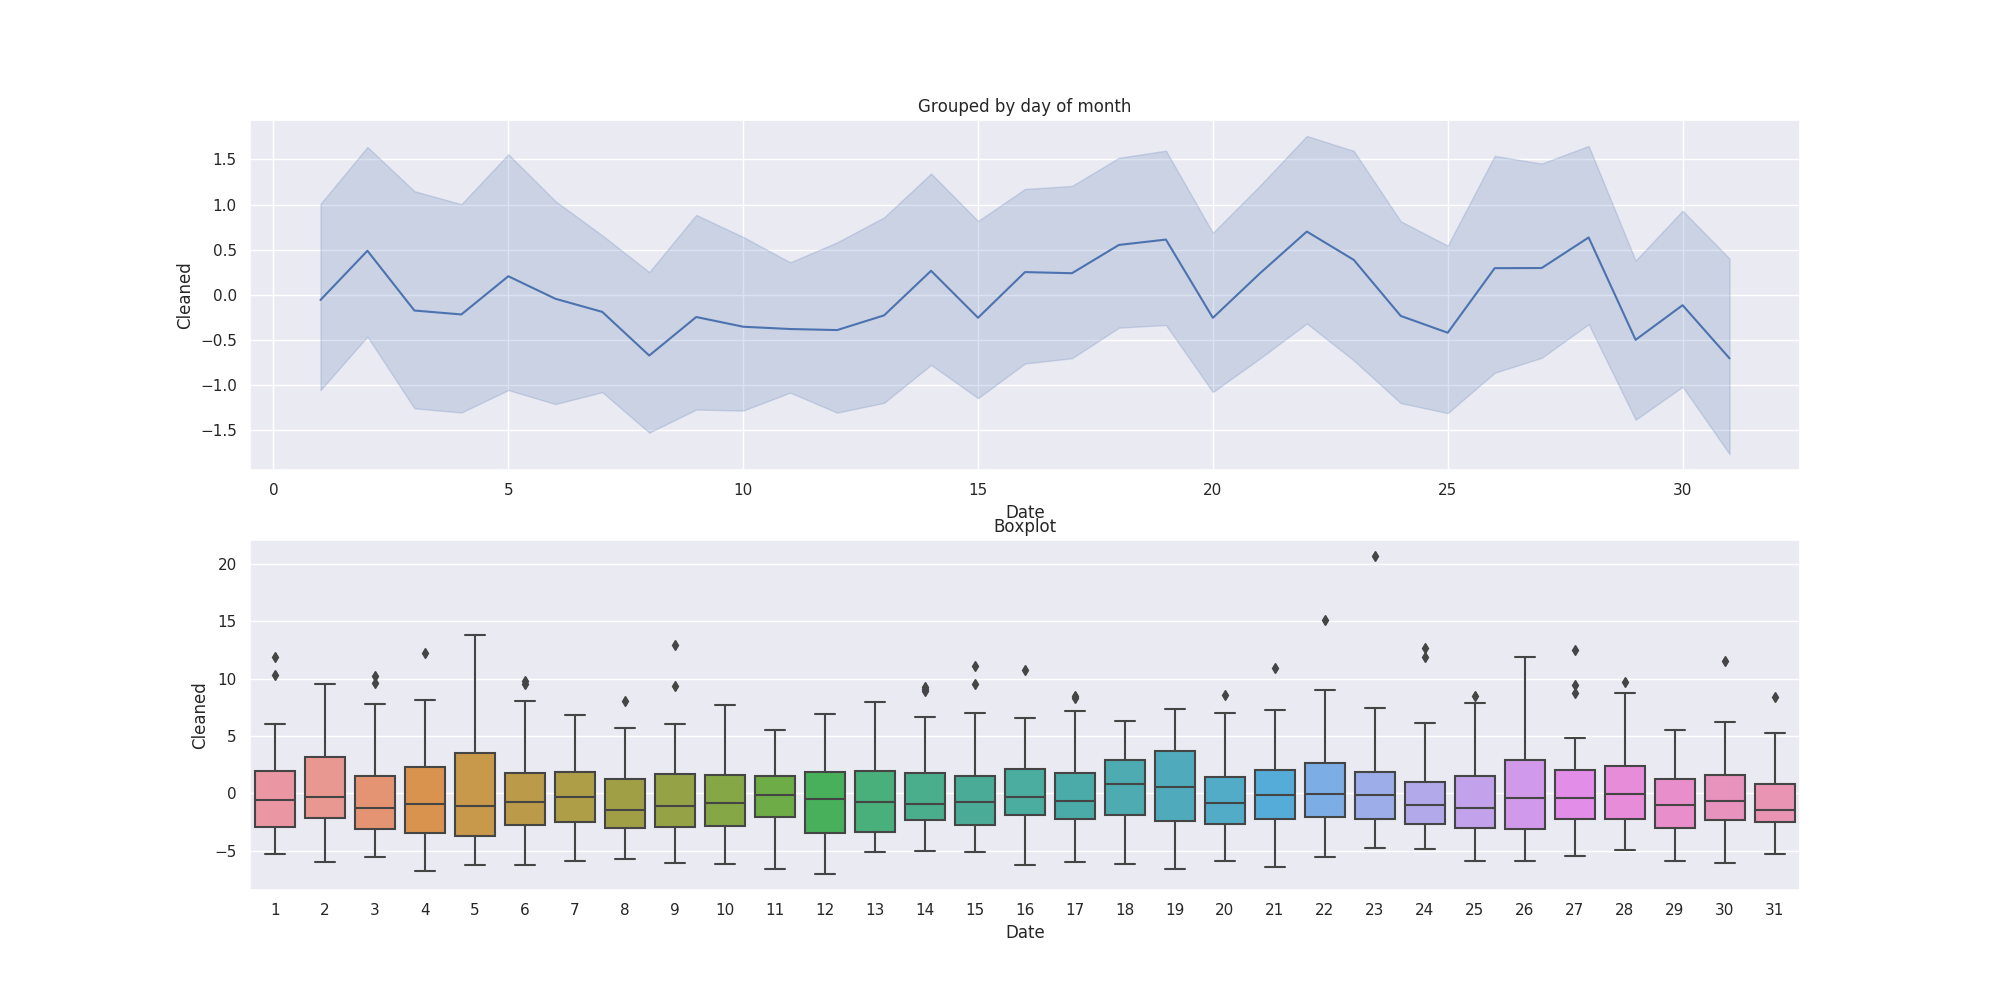
\includegraphics[width=0.7\textwidth]{plots/within_month.png}
  \caption{Retraso medio por d\'ia del mes}
  \label{fig:within_month}
\end{figure}

\begin{figure}[hbtp]
  \centering
  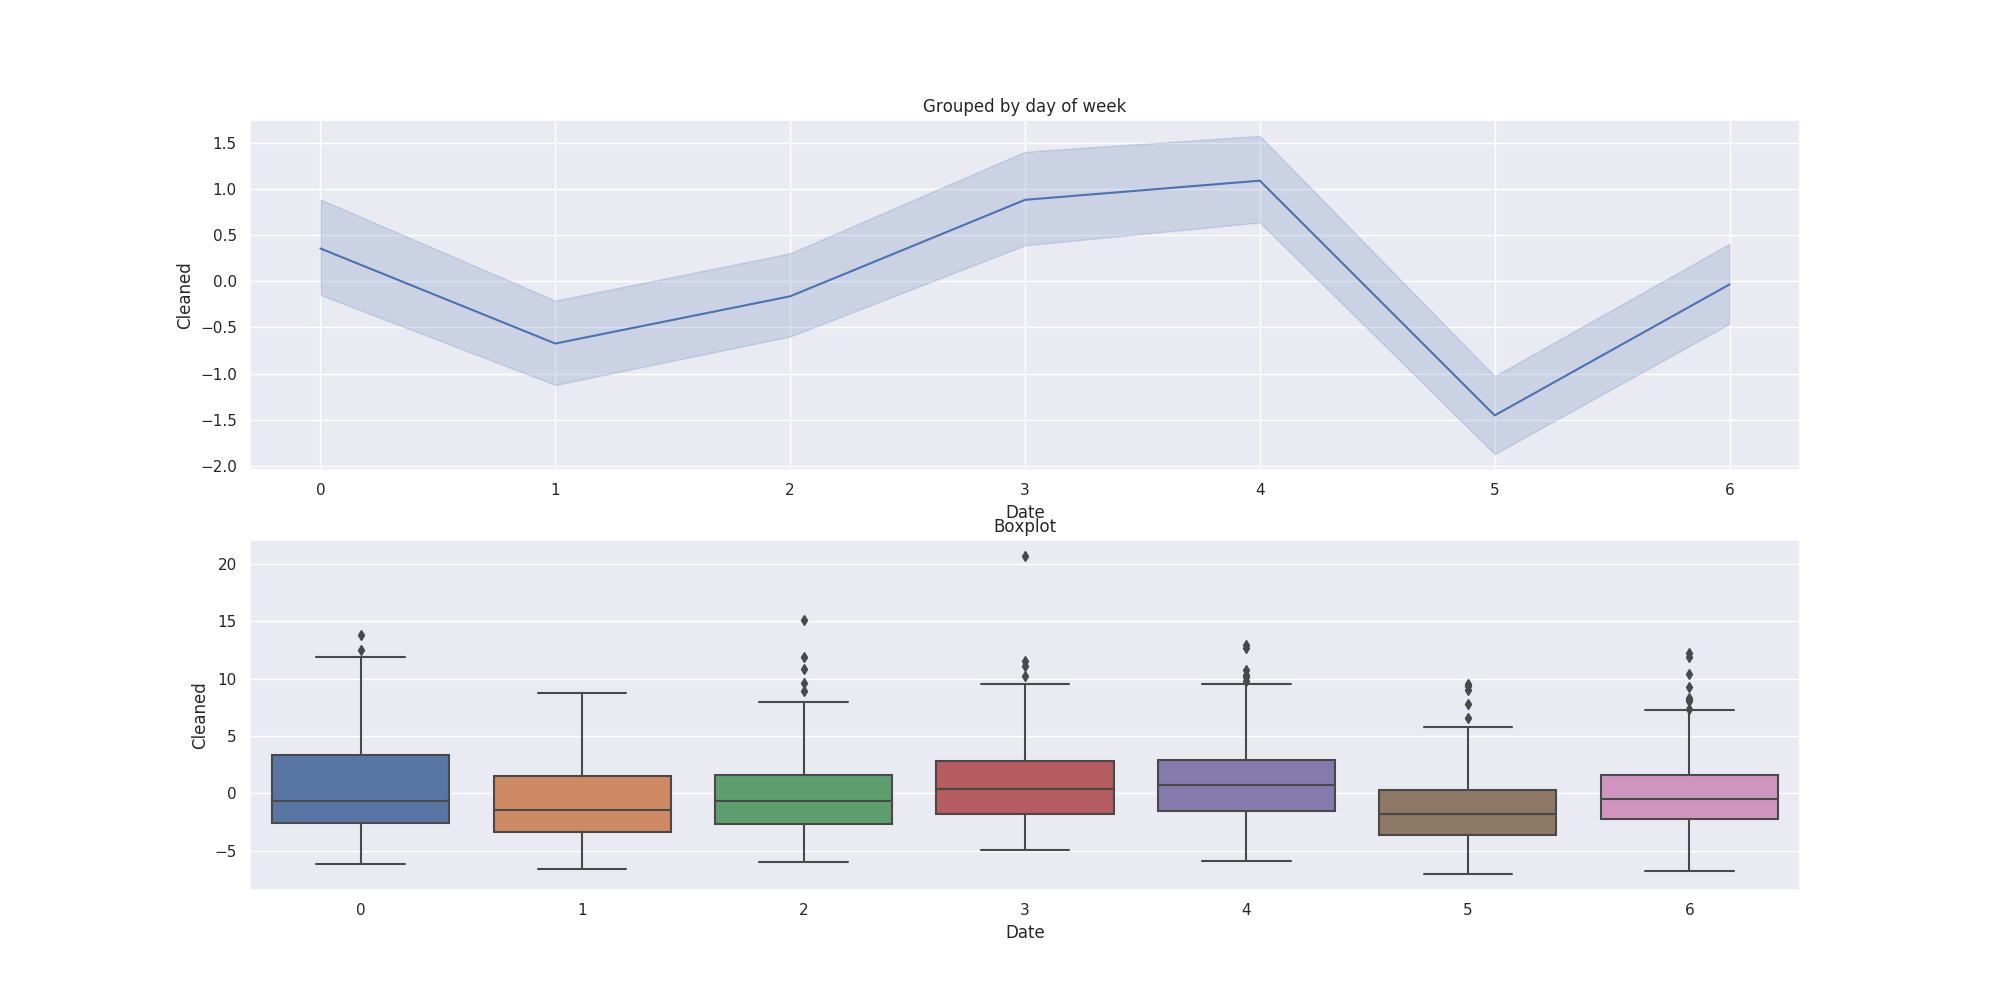
\includegraphics[width=0.7\textwidth]{plots/within_week.png}
  \caption{Retraso medio por d\'ia de la semana}
  \label{fig:within_week}
\end{figure}

Las figuras muestran un comportamiento peri\'odico de los retrasos. Es m\'as claro el de la figura \ref{fig:within_year}
que tiene elevaciones en los meses diciembre/enero y junio/julio, que es esperable pues son
meses de vacaciones. Tambi\'en se ve en la figura \ref{fig:within_week} un aumento en los d\'ias mi\'ercoles/jueves
y domingo/lunes. El comportamiento parece ser menos predecible para la figura \ref{fig:within_month}.

A modo de ejemplo, se muestran los m\'as altos scores
(explicados en la secci\'on \ref{subsec:scores}) del a\~no 2008
en las figuras \ref{fig:carrier_scores} y \ref{fig:airport_scores}.

\begin{figure}[hbtp]
  \centering
  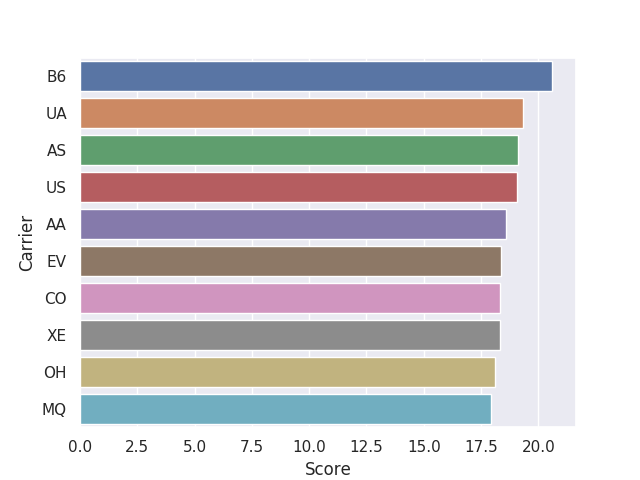
\includegraphics[width=0.6\textwidth, height=2in]{plots/carrier_scores_2008.png}
  \caption{Primeros puntajes de aerol\'ineas}
  \label{fig:carrier_scores}
\end{figure}

\begin{figure}[hbtp]
  \centering
  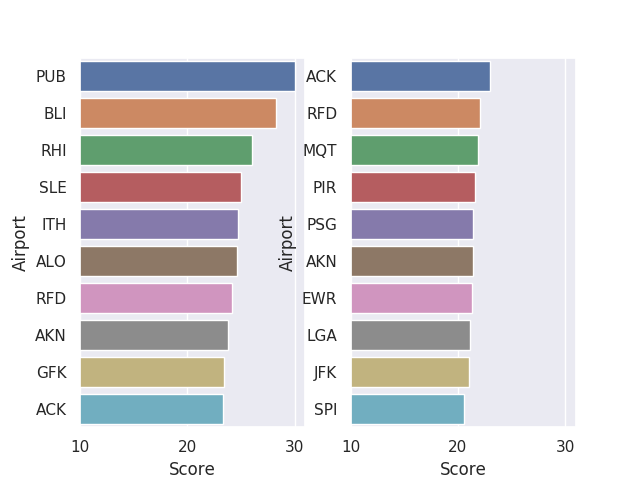
\includegraphics[width=0.7\textwidth, height=2in]{plots/airport_scores_2008.png}
  \caption{Primeros puntajes de aeropuertos (origen y destino)}
  \label{fig:airport_scores}
\end{figure}

Sobre la base de este an\'alisis se escogieron los features descritos en la secci\'on \ref{subsec:extraccion}.
Se ajust\'o un modelo de cuadrados m\'inimos (secci\'on \ref{subsec:prediction}).
En la figura \ref{fig:example_fit_prediction} se muestra el resultado del modelo con datos de entrenamiento
entre 2002 y 2006 y datos de test a partir de 2006.

\begin{figure}[hbtp]
  \centering
  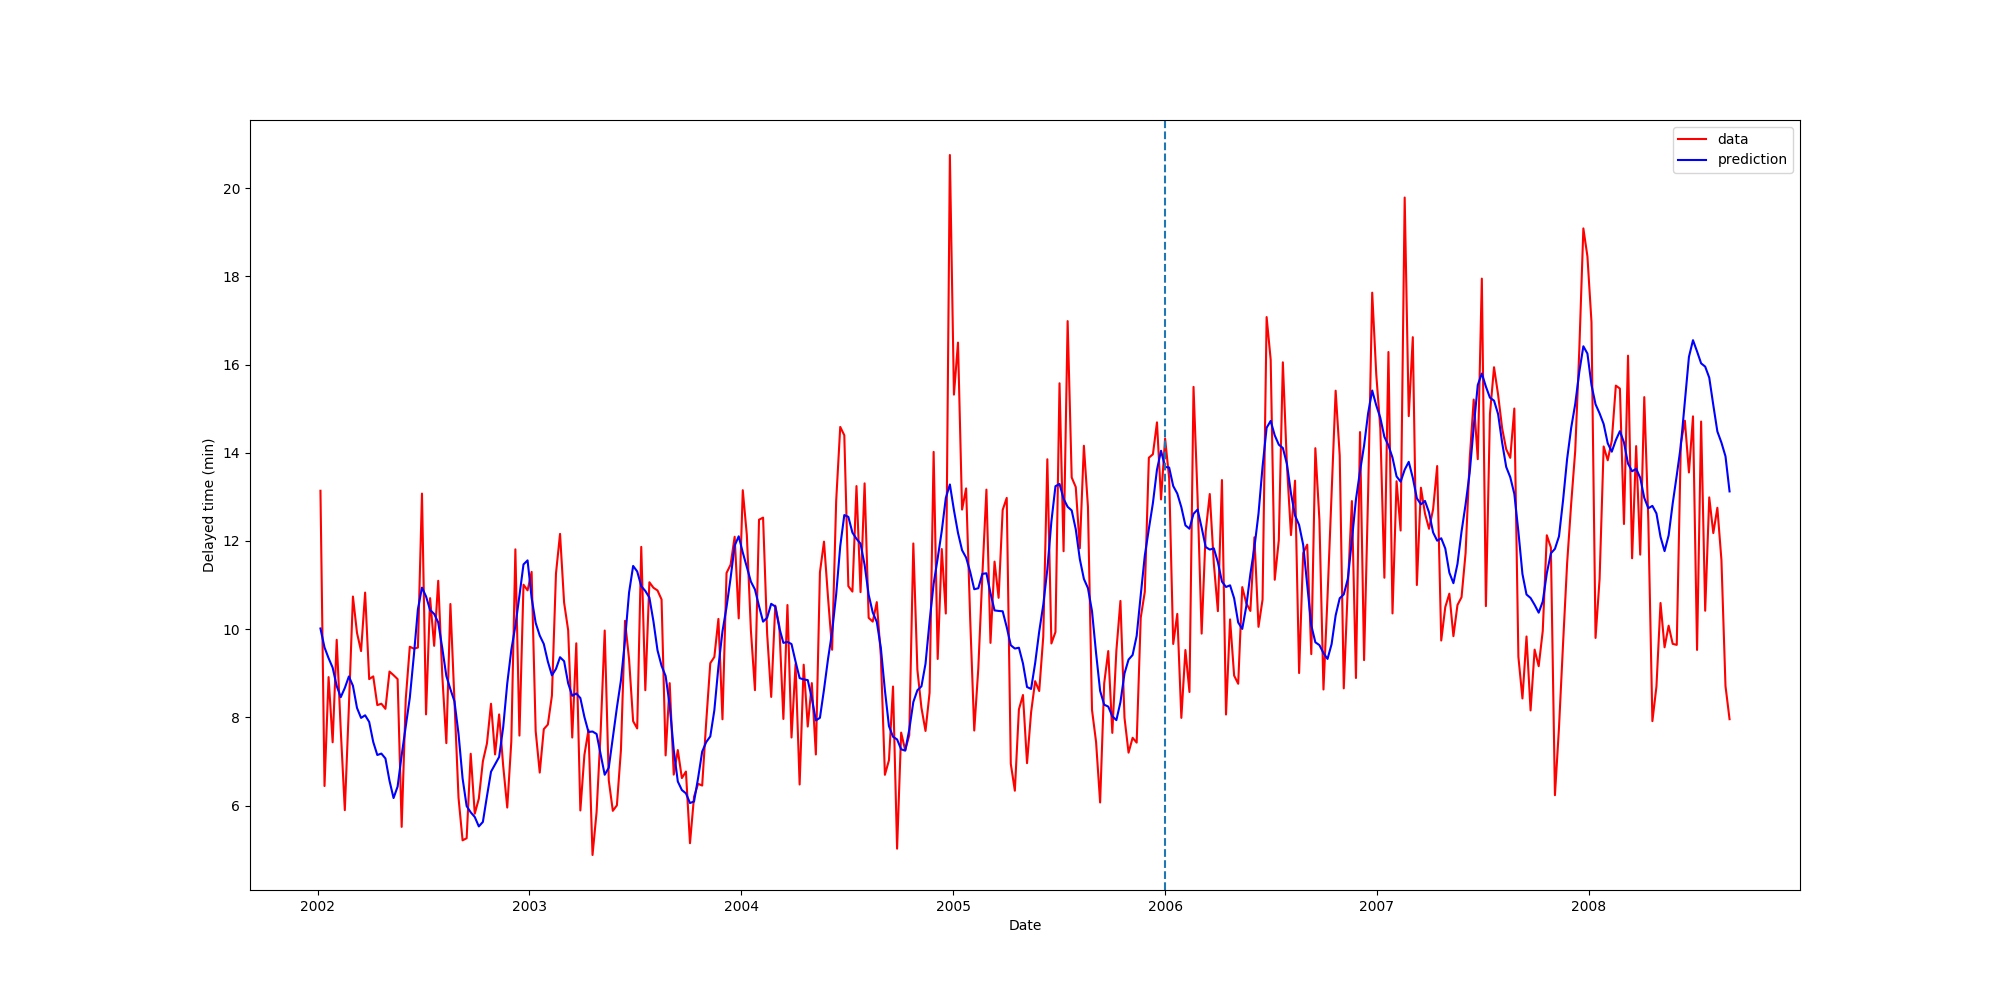
\includegraphics[width=\textwidth, height=3in]{plots/example_fit_and_prediction.png}
  \caption{Ejemplo de predicci\'on. La l\'inea punteada delimita el fin de los datos de
  entrenamiento y el comienzo de los datos de test}
  \label{fig:example_fit_prediction}
\end{figure}

Nos planteamos la pregunta: \textquestiondown Aprende el algoritmo efectivamente de los datos? \textquestiondown Mejora la predicci\'on si
entrenamos con m\'as datos? Para responder a esta pregunta, ejecutamos el modelo entrenando con una cantidad
creciente de a\~nos, desde uno a todos menos uno, y testeamos contra los dem\'as a\~nos. Exponemos
los resultados de las m\'etricas en la figura \ref{table:metrics}

\begin{figure}
\begin{center}
 \resizebox{\textwidth}{!}{%
  \begin{tabular}{||c || c | c | c | c | c | c | c||}
 \hline
 Training years & Delay RMSE & Delay NRMSE & RMSE & Accuracy & Precision & Recall & Balanced Accuracy \\ [1ex]
 \hline\hline
 1 & 14.19 & 0.24 & 0.53 & 0.72 & 0.32 & 0 & 0.5 \\
 \hline
 2 & 13.94 & 0.23 & 0.54 & 0.71 & 0.43 & 0 & 0.5 \\
 \hline
 3 & 14.01 & 0.23 & 0.57 & 0.68 & 0.42 & 0.21 & 0.54 \\
 \hline
 4 & 14.42 & 0.24 & 0.58 & 0.66 & 0.42 & 0.26 & 0.55 \\
 \hline
 5 & 14.62 & 0.24 & 0.59 & 0.65 & 0.42 & 0.27 & 0.55 \\
 \hline
 6 & 14.81 & 0.27 & 0.6 & 0.64 & 0.40 & 0.34 & 0.55 \\ [1ex]
 \hline
\end{tabular}}
\end{center}
\caption{M\'etricas para distintos datos de entrenamiento}
\label{table:metrics}
\end{figure}

Los resultados de las ejecuciones para distintos conjuntos de entrenamiento son parad\'ojicos, ya
que algunas m\'etricas mejoran (como Recall y Balanced Accuracy), pero otras empeoran
(como Delay NRMSE). Nuestra hip\'otesis es que se puede deber a que el modelo con m\'as datos
de entrenamiento es m\'as susceptible a \textit{overfitting}, o que al entrenar con conjunto de datos
m\'as grande se toma en consideraci\'on datos viejos que no son tan influyentes en los datos m\'as nuevos.

En la figura \ref{fig:flights_and_stock_prices} se grafican la cantidad de vuelos y el precio de las acciones
de algunas aerol\'ineas. En ella se puede ver algunas cosas notables, como por ejemplo el gran desplome
de los precios de las acciones con la crisis de 2008, o la aparici\'on importante de la aerol\'inea \texttt{AA},
y su ca\'ida en el 2008 a\'un m\'as grande que la de las otras aerol\'ineas.

\begin{figure}[hbtp]
  \centering
  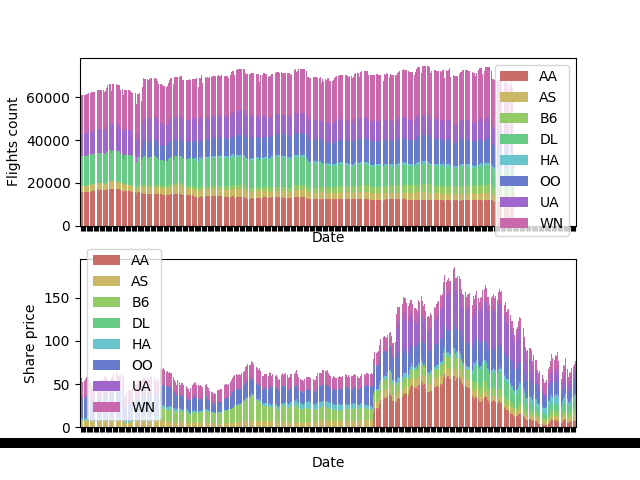
\includegraphics[width=0.7\textwidth, height=2.5in]{plots/flights_and_stock_prices.png}
  \caption{Cantidad de vuelos y precio de las acciones por aerol\'inea}
  \label{fig:flights_and_stock_prices}
\end{figure}

Una pregunta que nos planteamos es: \textquestiondown Est\'an correlacionadas ambas variables? Para
estudiarlo, consideramos, para cada aerol\'inea, qu\'e porcentaje de vuelos le corresponda a esa
aerol\'inea, y qu\'e porcentaje de precio de la acci\'on le corresponde (sobre el conjunto de aerol\'ineas para
las que tenemos datos de precios de acciones), y estudiamos la correlaci\'on (v\'ia coeficiente
de Pearson) de ambas variables a lo largo del tiempo. Exponemos los resultados del coeficiente de Pearson en la figura
\ref{table:pearson}. De la figura se desprende que no hay una correlaci\'on evidente entre estas variables,
ya que los valores del coeficiente de Pearson son variables entre 0.74 y -0.94.

\begin{figure}
\tiny
\begin{center}
  \begin{tabular}{||c || c ||}
 \hline
 Carrier & Pearson \\ [1ex]
 \hline\hline
 AA & 0.74 \\
 \hline
 AS & 0.33 \\
 \hline
 B6 & -0.94 \\
 \hline
 DL & 0.53 \\
 \hline
 HA & 0.05 \\
 \hline
 OO & -0.6 \\
 \hline
 UA & 0.29 \\
 \hline
 WN & -0.62 \\ [1ex]
 \hline
\end{tabular}
\end{center}
\caption{Coeficiente de Pearson entre el porcentaje de vuelos
y el porcentaje de precio de las acciones para cada aerol\'inea}
\label{table:pearson}
\end{figure}
